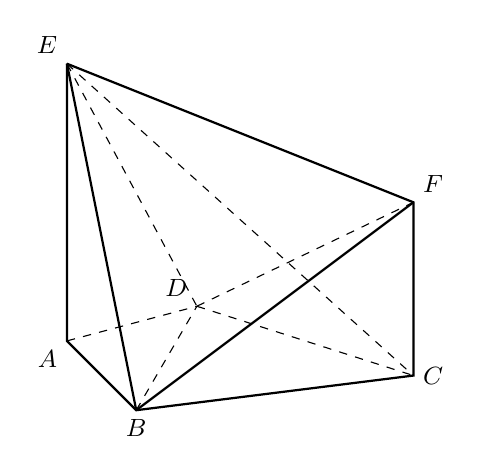
\begin{tikzpicture}[>=latex, font=\small, scale=1.1]
  % 顶点坐标
  \coordinate (A) at (0, 0);
  \coordinate (B) at (0.8, -0.8);
  \coordinate (C) at (4.0, -0.4);
  \coordinate (D) at (1.5, 0.4);
  \coordinate (E) at (0, 3.2);
  \coordinate (F) at (4.0, 1.6);

  % 虚线不可见边/内部对角线
  \draw[dashed, thin] (A) -- (D);
  \draw[dashed, thin] (D) -- (C);
  \draw[dashed, thin] (E) -- (D);
  \draw[dashed, thin] (E) -- (C);
  \draw[dashed, thin] (B) -- (D);
  \draw[dashed, thin] (D) -- (F);

  % 实线可见外轮廓与面边界
  \draw[thick] (E) -- (A) -- (B) -- (C) -- (F) -- (E);
  \draw[thick] (E) -- (B);
  \draw[thick] (B) -- (F);

  % 顶点标记
  \node[above left] at (E) {$E$};
  \node[below left] at (A) {$A$};
  \node[below] at (B) {$B$};
  \node[right] at (C) {$C$};
  \node[above right] at (F) {$F$};
  \node[above left] at (D) {$D$};
\end{tikzpicture}
